\section{Evaluation and judge audit}\label{sec:evaluation}
The judge (J1) combines open-vocabulary detection \citep{minderer2022owlvit} with CLIP colour classification \citep{radford2021clip} at pinned model revisions, with thresholds fixed before any test data (presence 0.10, count 0.15, size ratio 1.5). A second, question-answering judge was planned but not implemented and plays no role in any result.

\paragraph{Pre-declared audit.} A blinded, seeded, stratified sample of DEV (image, constraint) items was labelled by a human who saw only an opaque image and a neutral question (a colour, a count, a presence answer, which object is further left, or which looks larger), with ``not visible'' and ``ambiguous'' answers. Accuracy is population-weighted with a stratified bootstrap. A constraint type may carry a confirmatory claim only if its weighted accuracy is at least $0.85$; no other criterion was added after the data were seen.

\paragraph{Result.} Only presence met the criterion (Table~\ref{tab:dev-audit}, Figure~\ref{fig:audit}). The binding judge reached \accBind, count \accCount, spatial relation \accSpat{} (its sensitivity was low) and relative size \accSize. One annotator labelled the main package; a second package was labelled by the same person within the same session and is therefore neither an inter-rater nor a valid intra-rater check, and is not used. These limits are carried into every result (Section~\ref{sec:rq}).
% generated by paper/make_paper_assets.py from docs/evidence/audit_20261019/audit_verdicts.json
\begin{table}[t]
\centering\small
\caption{DEV evaluator audit of J1 against blinded human labels (one annotator; population-weighted accuracy, stratified bootstrap 95\% CI). Only types meeting $\geq 0.85$ may carry a confirmatory claim.}
\label{tab:dev-audit}
\begin{tabular}{lrrrr}
\toprule
Type & $n$ & Accuracy & 95\% CI & $\geq 0.85$ \\
\midrule
presence & 159 & 0.856 & [0.802, 0.907] & yes \\
count & 108 & 0.768 & [0.685, 0.843] & no \\
binding & 156 & 0.800 & [0.722, 0.871] & no \\
spatial & 109 & 0.615 & [0.523, 0.706] & no \\
size & 175 & 0.846 & [0.794, 0.897] & no \\
\bottomrule
\end{tabular}
\end{table}

\begin{figure}[t]\centering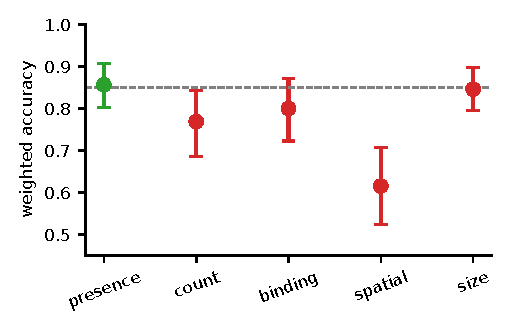
\includegraphics[width=0.55\linewidth]{figures/fig_audit.pdf}
\caption{Weighted accuracy of the automatic judge per constraint type on DEV (95\% bootstrap intervals; one annotator). Dashed line: pre-declared criterion $0.85$. Green: met; red: not met.}\label{fig:audit}\end{figure}
